\documentclass[journal,12pt,twocolumn]{IEEEtran}
\usepackage[utf8]{inputenc}
\usepackage{setspace}
\usepackage{gensymb}
\usepackage{tikz}
\usepackage{listings}
\usepackage{tkz-euclide}
%\doublespacing
\singlespacing
\usepackage[cmex10]{amsmath}
\usepackage{amsthm}
\usepackage{mathrsfs}
\usepackage{txfonts}
\usepackage{stfloats}
\usepackage{bm}
\usepackage{cite}
\usepackage{cases}
\usepackage{subfig}
%\usepackage{xtab}
\usepackage{longtable}
\usepackage{multirow}
%\usepackage{algorithm}
%\usepackage{algpseudocode}
\usepackage{enumitem}
\usepackage{mathtools}
\usepackage{tikz}
\usepackage{circuitikz}
\usepackage{verbatim}
\usepackage{tfrupee}
\usepackage[breaklinks=true]{hyperref}
\usetikzlibrary{calc,math}
\usepackage{listings}
\usepackage{color}                                            
\usepackage{array}                                           
\usepackage{longtable}                                      
\usepackage{calc}                                             
\usepackage{multirow}                                         
\usepackage{hhline}                                         
\usepackage{ifthen}                                          
\usepackage{lscape}     
\usepackage{multicol}
\usepackage{chngcntr}
\usepackage{enumerate}
\lstset{
%language=C,
frame=single, 
breaklines=true,
columns=fullflexible
}

\title{Exercise 8.1}
 
\author{Mohit Singh}
\date{21 May 2020}

\begin{document}
\maketitle{}


\begin{abstract}
This document provides the solution to the problem no. 36 given in the exercise 8.1. The problem is based on the congruence rules in triangles. The figures are provided using python and \LaTeX codes.
\end{abstract}

\noindent For figures, download the code from 
%
\begin{lstlisting}
svn co https://github.com/mohit-singh-9/Summer-2020.git
\end{lstlisting}
%
%and latex-tikz codes from 
%\begin{lstlisting}
%math/codes/tri_sss.py
%\end{lstlisting}

\section{PROBLEM No. 36}

\noindent Two sides AB and BC and median AM of one triangle ABC are respectively equal to sides PQ and QR and median PN of triangle PQR. Show that:
\newline
a) $\triangle ABM \cong \triangle PQN$
\newline 
b) $\triangle ABC \cong \triangle PQR$


\begin{figure}[!ht]
\centering
\resizebox{\columnwidth}{!}{%\documentclass{article}
%\usepackage[utf8]{inputenc}
%\usepackage{tikz}
%\usepackage{tkz-euclide}
%\begin{document}

\begin{tikzpicture}
[scale=1,>=stealth,point/.style={draw,circle,fill = black,inner sep=0.5pt},]

%Triangle sides
\def\a{6}
\def\b{5}
\def\c{6}
 
%Coordinates of A
\def\p{47/12}
%\def\p{4}
\def\q{{sqrt(\c^2-\p^2)}}

%Labeling points
\node (A) at (\p,\q)[point,label=above right:$A$] {};
\node (B) at (0, 0)[point,label=below left:$B$] {};
\node (C) at (\a, 0)[point,label=below right:$C$] {};

%Foot of perpendicular

\node (M) at (\a/2,0)[point,label=above right:$D$] {};

%Drawing triangle ABC
\draw (A) -- node[left] {$\textrm{c}$} (B) -- node[below] {$\textrm{a}$} (C) -- node[above,xshift=2mm] {$\textrm{b}$} (A);

%Drawing median AM
\draw (A) -- node[left] {$\textrm{}$}(M);

%Drawing and marking angles
\tkzMarkAngle[fill=orange!40,size=0.5cm,mark=](C,B,A)
\tkzLabelAngle[pos=-0.9](A,B,C){$\alpha$}

\end{tikzpicture}

\begin{tikzpicture}
[scale=1,>=stealth,point/.style={draw,circle,fill = black,inner sep=0.5pt},]

%Triangle sides
\def\p{6}
\def\q{5}
\def\r{6}
 
%Coordinates of P
\def\x{47/12}
%\def\p{4}
\def\z{{sqrt(\r^2-\x^2)}}

%Labeling points
\node (P) at (\x,\z)[point,label=above right:$P$] {};
\node (Q) at (0, 0)[point,label=below left:$Q$] {};
\node (R) at (\p, 0)[point,label=below right:$R$] {};

%Foot of median

\node (N) at (\p/2,0)[point,label=above right:$N$] {};

%Drawing triangle PQR
\draw (P) -- node[left] {$\textrm{r}$} (Q) -- node[below] {$\textrm{p}$} (R) -- node[above,xshift=2mm] {$\textrm{q}$} (P);

%Drawing median PN
\draw (P) -- node[left] {$\textrm{}$}(N);

%Drawing and marking angles
\tkzMarkAngle[fill=orange!40,size=0.5cm,mark=](R,Q,P)
\tkzLabelAngle[pos=-0.9](P,Q,R){$\theta$}

\end{tikzpicture}
%\end{document}
}
\caption{$\triangle ABC$ and $\triangle PQR$ using Latex}
\label{fig:triangle_latex}
\end{figure}
\begin{figure}[!ht]
\centering
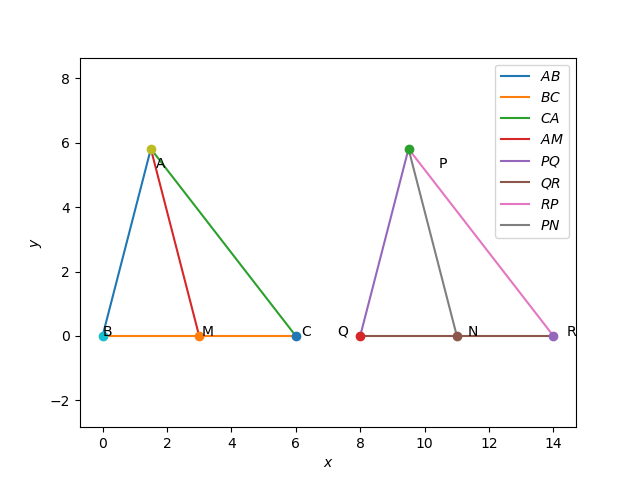
\includegraphics[width= \columnwidth]{Figure_1.png}
\caption{$\triangle ABC$ and $\triangle PQR$ using Python}
\label{fig:triangle_python}
\end{figure}


\section{CONSTRUCTION}
Download the python code from
\begin{lstlisting}
./codes/triangle_python.py
\end{lstlisting}
and latex code from
\begin{lstlisting}
./fig/triangle_fig.tex
\end{lstlisting}

The triangles in the Fig \ref{fig:triangle_latex} and Fig \ref{fig:triangle_python} are constructed with the following length of sides:
\newline
In $\triangle ABC$: AB = BC = 6 cm , AC = 5 cm. M is the midpoint of BC. So, AD is the median.
\newline
In $\triangle PQR$: PQ = QR = 6 cm , PR = 5 cm. N is the midpoint of QR. So, PN is the median.




\section{SOLUTION}

\noindent a) \\
    In $\triangle ABM$  and  $\triangle PQN$ \newline 
    AB = PQ (Given)  \newline
    AM = PN (Given) \newline
    Since M and N are midpoints and BC = QR , \newline
    BM = QR  \newline
    :. By SSS congruence rule , $\triangle ABM \cong \triangle PQN$  \newline
    
        So now $\angle ABM = \angle PQN$ i.e $\alpha = \theta$
    \newline
    \\
    \\
b) \\   
Now in $\triangle ABC$  and  $\triangle PQR$ \newline 
AB = PQ (Given)  \newline
$\alpha = \theta$ \newline
BC = QR (Given)\newline
:. By SAS congruence rule , $\triangle ABC \cong \triangle PQR$ 
    




\end{document}
